\section{Introduction}
\label{sec:1-introduction}
%% Labels are used to cross-reference an item using \ref command.

Maintenance scheduling is part of a class of operational problems that have proven hard to solve (NP-hard~\citep{garey1979computers}).
Furthermore, for optimization to be utilized if the dynamic and uncertain environment where maintenance scheduling 
is performed requires a
tight integration with third party administration software to enable the tacit knowledge of decision makers to influence
the planning process easily. Often a number of different decision makers at different company levels take part in the
planning process and in this way the industry usually assigns responsibility for decision-making to an individual
representing only a small part of the complete process.  These multiple smaller planning processes are often difficult
to map to a single mathematical model describing the whole system as elaborated by~\citep{barthelemy2002human}. Solving
operation research problems that are operational in nature have additional requirements over more typical static
problems: they have to be responsive to changing parameters; able to be assimilated into the decision-makers workflow;
allow for integration with dynamic data sources such as databases and APIs~\citep{meignan_review_2015}. Operational
aspects of operation research, as opposed to higher level strategic and tactical aspects, are characterized by extensive
amounts coordination and negotiation on proposed schedules. The lack of integration and responsiveness can lead to schedules
that are not directly implemented in practice but instead provides initial suggestions~\citep{meignan_review_2015},
which are then iterated on elsewhere in the scheduling process. In~\citep{barthelemy2002human} the authors
argue that many problems that operation research aim to solve are often composed of a group of individuals
whose decisions are consolidated into an "epistemic subject" for which a mathematical model can be formulated
and solved, with many scheduling problems being good examples. However often multiple actors have different
views on what constitutes an optimal schedule hence resulting in multiple-objectives. Even if multi-objective
optimization~\citep{ehrgott2002multiple} is applied to find the Pareto Front~\citep{Pareto1897} a negotiating process
still is needed between the actors to select the final schedule. This paper proposes a solution method that will allow
for real-time optimization based on actor/user interaction and connection to a dynamic data source, effectively managing
the changes to the parameter space. The proposed solution method will be tested on the multi-compartment multi-knapsack
problem (MCMKP) for maintenance scheduling on a large dataset from a company. The MCMKP naturally models what in
the practical maintenance is called the weekly schedule, taken form \citep{palmerMaintenancePlanningScheduling2019}.
It should be noted that the scientific maintenance scheduling literature deviates significantly from its practical
implementation which is also detailed in \citep{palmerMaintenancePlanningScheduling2019}. The solution method will by
based on the large neighborhood search (LNS) metaheuristic. This meta heuristic was chosen due to its properties
of naturally being able to work with and fix infeasible solutions and its state of the art performance on various
scheduling problems. \citep{???} To understand the need for actor-based methods some background knowledge will be required about
the maintenance scheduling process. In figure \ref{fig:integrated:maintenance-process} illustrates the general setup of
a healthy maintenance planning and scheduling system. The system's actors have the following responsibilities: the
planner generates the work orders that are to be scheduled; the scheduler creates weekly schedules based on a knapsack
formulation; based on the weekly schedule the supervisor assigns work order activities that the work order is composed
of (the assignment problem); the technicians executes the work in sequential pattern (single machine scheduling).
A final point on the necessity of actor-based approaches to model should a setup is the idea of ownership of a work
order. Throughout the scheduling process a work order is owned by a specific actor and he alone is allow to modify
it. This means that a single model approach is very difficult to implement in practice as a work order is modelled
differently depending on the actor that currently owns it. This also highlight another an point in maintenance scheduling: that
the stochastic nature of the maintenance scheduling process can be handled using a change of model each with different
levels of aggregation and different sets of constraints, opposed to more academic approaches such as fuzzy logic and 
stochastic optimization. When the fundamental uncertainties manifest themselves during planning or execution work orders
are rescheduled by moving between the different actor (models), meaning that the stochastic elements of maintenance 
scheduling are handled by dynamic rescheduling between the actors.

\begin{figure}
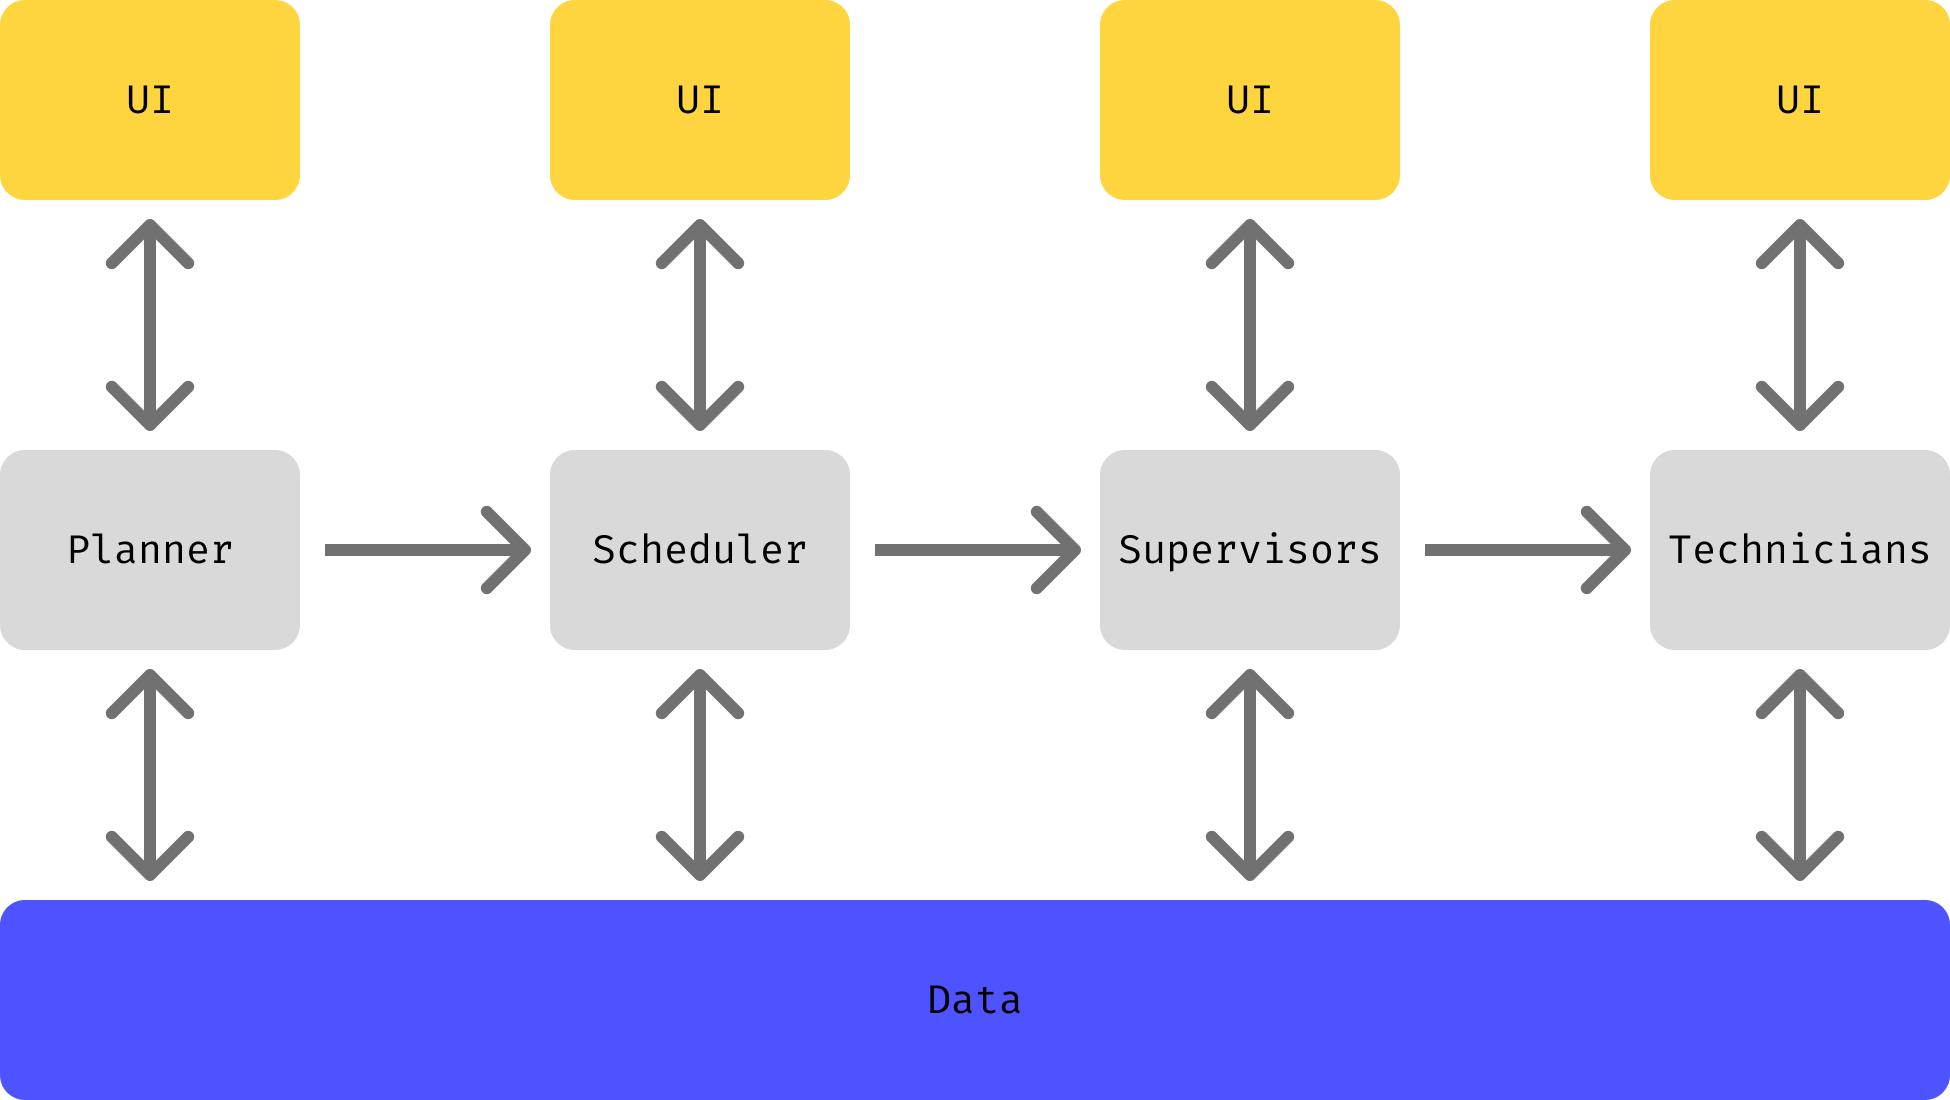
\includegraphics[width=1.0\textwidth]{figures/Scheduling Process Integrated.png}
\caption{Simple overview of the scheduling process with its primary types of actors. The planner, the scheduler, the supervisor(s), and the technicians. 
The green color highlights the scheduler as it the actor in the maintenance scheduling process that is the foundation for the paper.}
\label{fig:simple-maintenance-process}
\end{figure}

This article describes a number of contributions: 

\begin{itemize}
\item A specialized LNS metaheuristic to be utilized in an actor framework
\item An actor based metaheuristic framework
\item Implementation and test on a large realworld maintenance scheduling problem
\end{itemize}

The paper is divided into four different sections. Section \ref{sec:2-solution-method} explains the weekly maintenance scheduling model in detail and forms the fundation of the paper. Section \ref{sec:3-results} shows that results coming from the implemented system where the implementation will be affected by simulated user-interaction. Section \ref{sec:4-discussion} will discuss the implications of the research and possible future research directions.

\subsection{A generic maintenance scheduling model}
\label{sub2sec2}
A large company needs to create a weekly maintenance plan for the next $p \in P$ weeks. The maintenance plan is planned centrally and consists of scheduling the $w \in W$ work orders, i.e. maintenance tasks, such that all are scheduled into different weeks. Each work order requires some resourses to be carried out, e.g. man-power with different qualifications, equipment etc. all of these resourses are available in limited amounts and are called traits $\tau \in T$. To simplify matters, we will assume that the recourse limits are not hard but extra workers can be paid overtime, extra equipment can be rented etc., at the cost (penalty) of $pen_{p\tau}$. The urgency of the different maintenance operations varies and is reflected in a penalty for carrying out a maintenance work order in a certain week $v_{wp}(t)$. Urgent tasks have quickly increasing penalties for the later weeks week $p$. Furthermore, two sets exists which will either will require the work order to be carried out in week $p$, i.e. $(w,p) \in E$ and a set which forbids a work order to carried out in week $p$, i.e. $(w,p) \in I$. The model for the problem is the Multi-compartment Multi-knapsack Problem with capacity penalties MCMKP.

The notation used in the model is based on the notation from the dynamic metaheuristics literature as found in \cite{yangMetaheuristicsDynamicCombinatorial2013}, where $t$ is added as a time variable on all sets, parameters, and variables that are subject to change.
This allows us to be precise in the timing on the messages that are send to the Ab-LNS.  

%\subsection{The Weekly Schedule: Multi-compartment Multi-knapsack Problem with capacity penalties}
%\label{sub2sec2}
%The actor-based large neighborhood search is implemented on the MCMKP which models that weekly schedule in maintenance. The model is comprised of five different sets. $P$ is the number of weekly periods; $W$ is the number of work orders; $\tau$ is the number of different traits; $E$ is a set that defines which work orders should be excluded from a specific weekly period; $I$ is an inclusion set that defines the allocation of specific work orders which should be included in a specific weekly period. The model has four parameters. $v_{pw}$ is the value of work order $w$ in weekly period $p$; $d$ is the penalty for exceeding a specific trait capacity; $c_{w\tau}$ is the capacity requirement for work order $w$ for trait $t$; $cap_{p\tau}$ is the total amount of capacity available in for weekly period p for for trait t. The model has 2 decision variables. $x_{wp}$, is a binary decision variable equal to one if work order w is in weekly period p and zero otherwise; $pen_{p\tau}$ is non-negative decision variable equal to the amount of excess capacity above the $cap_{p\tau}$ in weekly period p for trait $\tau$. The parameters $v$, $cap$, $Q$, and $P$ are functions of time, $\tau$, in this case as they will be subject to change during the solution process.


\newpage
\begin{alignat}{2}
	& \text{\rule{\linewidth}{0.4pt}} \notag\\
	& \textbf{Meta variables:} \notag\\
	& \ElementScheduler \in \SetScheduler \\
	& \VarTacticalWork{}{} \\ 
	& \tau \in [0, \infty] \\
	& \text{\rule{\linewidth}{0.4pt}} \notag\\
	& \textbf{Minimize:} \notag                                                                                                                                                        \\
	& \sum_{\ElementWorkOrder \in \SetWorkOrder{}} \sum_{\ElementPeriod \in \SetPeriod} \ParStrategicValue \cdot \VarStrategicWorkOrderAssignment{\ElementWorkOrder}{\ElementPeriod}  \notag\\ 
	& + \sum_{\ElementPeriod \in \SetPeriod} \sum_{\ElementResource \in \SetResource} \ParStrategicPenalty \cdot \VarStrategicExcess     \notag                                              \\
	& + \sum_{\ElementPeriod \in \SetPeriod} \sum_{\ElementWorkOrder1 \in \SetWorkOrder{}} \sum_{\ElementWorkOrder2 \in \SetWorkOrder{}} 	 \quad \ParClusteringValue \cdot \VarStrategicWorkOrderAssignment{\ElementWorkOrder1}{\ElementPeriod} \cdot \VarStrategicWorkOrderAssignment{\ElementWorkOrder2}{\ElementPeriod}  \\
	& \text{\rule{\linewidth}{0.4pt}} \notag\\
	& \textbf{Subject to:} \notag                                                                                                                                                      \\
	& \sum_{\ElementWorkOrder \in \SetWorkOrder{}} \ParStrategicWorkOrderWeight \cdot \VarStrategicWorkOrderAssignment{\ElementWorkOrder}{\ElementPeriod} \leq \ \ParStrategicResource + \VarStrategicExcess                                                                           \quad \forall \ElementPeriod \in \SetPeriod \quad \forall \ElementResource \in \SetResource                                                                                      \\
	& \sum_{\ElementWorkOrder \in \SetWorkOrder{}} \VarStrategicWorkOrderAssignment{\ElementWorkOrder}{\ElementPeriod} = 1              \quad \forall \ElementPeriod \in \SetPeriod                                                                                                                                      \\
	& \VarStrategicWorkOrderAssignment{\ElementWorkOrder}{\ElementPeriod} = 0                                                            \quad \forall (\ElementWorkOrder, \ElementPeriod) \in \ParStrategicExclude                                                                                                       \\
	& \VarStrategicWorkOrderAssignment{\ElementWorkOrder}{\ElementPeriod} = 1                                                            \quad \forall (\ElementWorkOrder, \ElementPeriod) \in \ParStrategicInclude                                                                                                       \\
	& \VarStrategicWorkOrderAssignment{\ElementWorkOrder}{\ElementPeriod} \in \{0, 1\}                                                   \quad \forall \ElementWorkOrder \in \SetWorkOrder{} \quad \forall \ElementPeriod \in \SetPeriod                                                                                 \\ 
	& \VarStrategicExcess \in \mathbb{R}^{+}                                                                                             \quad \forall \ElementPeriod \in \SetPeriod \quad \forall \ElementResource \in \SetResource                                                                                  \\ 
	& \text{\rule{\linewidth}{0.4pt}} \notag
\end{alignat}
\newpage



The objective function \eqref{eqn:objective_function_strategic_value}, \eqref{eqn:objective_function_strategic_penalty}, and
\eqref{eqn:objective_function_strategic_clustering}
minimizes the total weighted delay of all work order assignments together
with the penalty $\ParStrategicPenalty$ for exceeding the resource capacity given in constraint
\eqref{eqn:capacity_constraint}. The thrid term  
of the model contains the $\ParClusteringValue$ which turns the model into a 
quadratic problem. This term optimizes the value of putting two work orders
in the same period, if they have share similarity like close proximity, 
same functional location, etc. 

Constraint \eqref{eqn:capacity_constraint}
ensures that all the weights $\ParOperationWork{wr}$ for each activity in an work
order, given that it has been assigned, is lower than the capacity for each
period and for each trait $\tau$. $pen_{p\tau}$ is the amount of exceeded
capacity that is needed for the current assignment of work order to be
feasible. Constraint \eqref{eqn:single_workorder_constraint} makes sure
that each work order is assigned to at least a single period. Constraint
\eqref{eqn:exclusion_constraint} excludes a work order from a certain period
and constraint \eqref{eqn:inclusion_constraint} forces a specific work order
to be in a specific period. Constraint \eqref{eqn:x_integrality_constraint} and
\eqref{eqn:p_non_negativity_constraint} specify the variable domain for $x_{wp}$
and $pen_{p\tau}$ respectively. The effects of changing $E$, $I$, $cap$, and $v$
in real-time will be examined to determine their effects on the weekly schedules
and objective value.

The objective function \eqref{eqn:objective_function_strategic} minimizes the total weight of all work order assignments together with the penalty $d$ for exceeding the capacity given in constraint \eqref{eqn:capacity_constraint}. Constraint \eqref{eqn:capacity_constraint} ensures that all the weights $c_{w\tau}$ for each activity in an work order, given that it has been assigned, is lower than the capacity for each period and for each trait $\tau$. $pen_{p\tau}$ is the amount of exceeded capacity that is needed for the current assignment of work order to be feasible. Constraint \eqref{eqn:single_workorder_constraint} makes sure that each work order is assigned to at least a single period. Constraint \eqref{eqn:exclusion_constraint} excludes a work order from a certain period and constraint \eqref{eqn:inclusion_constraint} forces a specific work order to be in a specific period. Constraint \eqref{eqn:x_integrality_constraint} and \eqref{eqn:p_non_negativity_constraint} specify the variable domain for $x_{wp}$ and $pen_{p\tau}$ respectively. The effects of changing $E$, $I$, $cap$, and $v$ in real-time will be examined to determine their effects on the weekly schedules and objective value.
